% !TeX root = ../../thesis.tex


%overview of the methodology to be used;
% ~20 pages

\chapter{Methods}
\label{chap:methods}

This chapter discusses why the semantic web will be used for creating a semantic knowledge base of sensor metadata based on the studies and standards that have been reviewed in Chapter \ref{chap:rw} (Section \ref{par:LDmetadata}). Afterwards, a number of methods and standards are presented which are required for creating a semantic knowledge base, such as a method for creating linked data (Section \ref{par:missier}), observation data ontologies based on \ac{om} (Section \ref{par:ontologies2}), a method for creating inward links using DBPedia (Section \ref{par:dbpedia}) and two implementations of spatial query functions in \ac{sparql} (Section \ref{par:SpatialFilters}). The last part of this chapter describes the \ac{ogc} standard for web services containing online processes: the \acf{wps} (Section \ref{par:wps}). Chapter \ref{chap:design} presents a conceptual system architecture based on these methods. 

\section{Creating linked data}
\label{par:missier}
For publishing sensor data on the semantic web a conversion of this data to \ac{rdf} is required. For this the method by \cite{LD:Missier} will be reused. She developed a workflow for publishing linked open data, using existing spatial data as input (Figure \ref{fig:missier}). This workflow consists of three phases: preparation, modelling and conversion. The next subsections will describe these three phases in more detail.

\begin{figure}
	\centering
	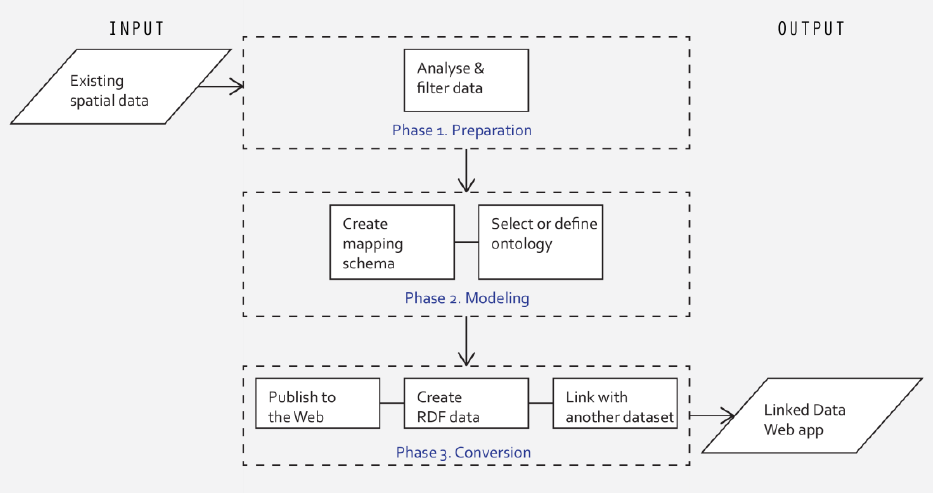
\includegraphics[width=1\linewidth]{UML/workflowMissier.png}
	\caption{Workflow diagram for publishing linked open data from existing spatial data \citep[p. 28]{LD:Missier}}
	\label{fig:missier}
\end{figure}

\subsection{Phase 1: Preparation}
The preparation phase is concerned with data acquisition, analysis and filtering. After an acquired dataset has been selected to convert to linked data it should be carefully examined. When creating linked data it is important to know the content and format of the input data. \cite{LD:Missier} explains that this understanding of the data is crucial for selecting the right ontologies and using the right software tools to process the data. Data filtering should be performed to select the parts of the dataset that need to be mapped to linked data. In this step the data quality could also be improved if necessary. The result of this phase should be a clean dataset with semantics about the content. This content has been filtered to only contain the parts of data which are required as linked data. 
 
\subsection{Phase 2: Modelling}
In modelling data to linked data the first step is to select an ontology. An ontology is part of a data model, that contains semantics of how objects in the real world are mapped inside a dataset. To improve interoperability it is preferred to (re)use an already existing ontology. Ontologies that have been implemented by others can be found in the Linked Data Cloud (\url{http://lod-cloud.net/}), which is an overview of linked data sets. Newly developed ontologies can be found via an analysis of academic literature. However, if there is no suitable ontology available a new one should be created. To select an ontology all ontologies that describe the type of data inside the dataset should be listed. The one that fits the dataset and the final application best should be selected. A mapping schema can be created to link parts of the data to their corresponding classes in the ontology. \cite{LD:Missier} stresses that it is also important to reuse common predicates associated with an ontology. This makes the data more understandable and it is easier to merge with other datasets using the same ontology and predicate. 

\subsection{Phase 3: Conversion}
In the conversion of data to linked data \cite{LD:Missier} describes two approaches: the \ac{rdf} storage approach and the `on-the-fly' conversion. In the first approach data is converted to linked data and stored in a triple store. This triple store can be queried by a \ac{sparql} endpoint. Alternatively, data can be stored in a spatial database and converted to \ac{rdf} on the fly when it is requested. There are advantages and disadvantages to both methods. On the one hand, creating a triple store creates duplicate data, which should be very well maintained to prevent the duplicate data being out of sync. On the other hand creating a triple store is a one time operation after which the querying with \ac{sparql} is quite efficient. The on-the-fly conversion does not create duplicate data, but has to convert its data to \ac{rdf} for every \ac{sparql} query.

\section{Ontologies}
\label{par:ontologies2}
\begin{sloppypar}
To publish data on the semantic web ontologies are required to specify the different classes and their relations. From the \ac{uml} diagram in Figure \ref{fig:OM_observation} the classes \texttt{Process}, \texttt{ObservedProperty} and \texttt{FeatureOfInterest} can be mapped to classes belonging to \ac{owl} for observations \citep{SSW:Cox}. Instances of \acp{foi} can be a \texttt{SamplingFeature} and a \texttt{SamplingPoint}. These can be mapped to classes from \ac{owl} for sampling features \citep{SSW:Cox2}. The PROV ontology can be used to describe changes in metadata for the \texttt{sensor} and \texttt{SensorObservationService} classes \citep{LD:W3C2}. These ontologies will be described in more detail in the next subsections.
\end{sloppypar}

\subsection{Observation metadata}
In Section \ref{par:ontologies} a number ontologies are described that define observations. The evaluation of observation metadata ontologies by \cite{SW:Hu} is interesting, since it exposes what the relevant aspects are in the process of observation discovery. However, their proposed model focusses mainly on including remote sensing and imagery data in metadata models that were not originally created for this kind of data. The \ac{ssno} is an ontology that clearly describes the process between sensor, stimulus and observation. However, \cite{SSW:Cox4} points out that an important aspect of describing a sensor network is missing in this ontology: the sampling. Also, the om-lite and sam-lite ontologies by \cite{SSW:Cox4} are lightweight ontologies that can be complemented by already existing linked data ontologies. They do not rely on the (heavy) \ac{iso} specifications that date from before the semantic web, unlike the \ac{ssno}. The om-lite and sam-lite ontologies will therefore be used in this thesis. 

\subsection{Provenance}
\cite{SSW:Cox4} describes that the PROV ontology can be used in combination with om-lite to keep track of changes in observation metadata. This `PROV-O' aims to semantically define the concepts behind provenance in linked data. Provenance has to do with changes that occur over time. This ontology allows the definition of Entities, Activities and Agents. Figure \ref{fig:PROV} shows the relations between  Entities, Activities and Agents. An Entity is a physical, digital, conceptual, or other kind of (real or imaginary) thing. An Activity is something that takes place over a period of time and acts with entities. An Agent is something that is in some way responsible for an activity taking place, an entity existing, or for another agent's activity. 

\begin{figure}
	\centering
	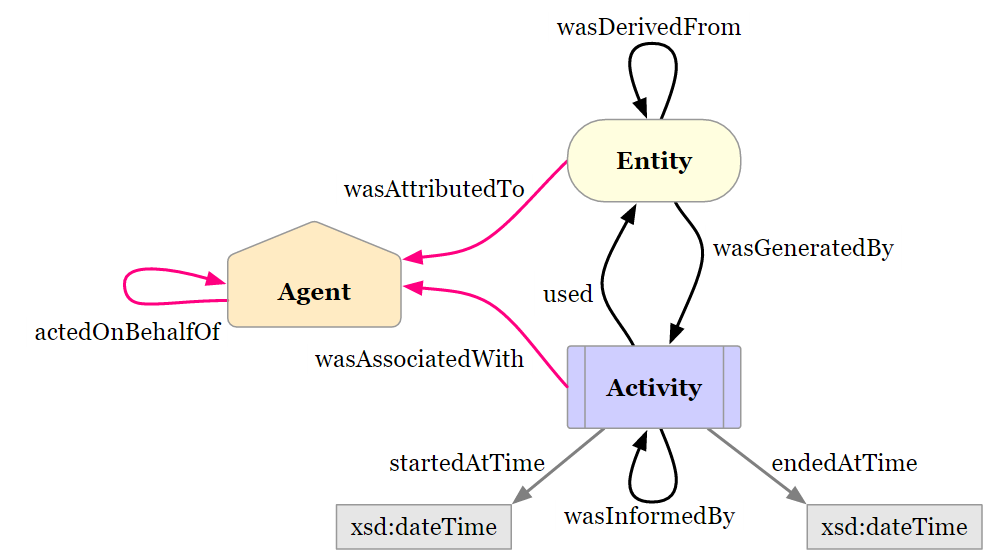
\includegraphics[width=1\linewidth]{UML/PROV.png}
	\caption{Basic classes and relations in the PROV-O by \citep{LD:PROV}}
	\label{fig:PROV}
\end{figure}

\section{Adding links to DBPedia}
\label{par:dbpedia}

\begin{sloppypar}
	For adding outgoing links to their semantic knowledge base, DBPedia has created a GitHub repository called `dbpedia-links' (\url{https://github.com/dbpedia/links}). The steps that should be followed to add links are described here, together with examples. The first step in establishing DBPedia links is to create an \ac{rdf} file containing the links to be added. The subjects of these triples should be a DBPedia \ac{iri}, using either the main namespace \url{http://dbpedia.org/resource} or one of its \url{ http://xxx.dbpedia.org/resource} subdomains, such as \url{http://nl.dbpedia.org/resource}. The predicates in this file can be: \texttt{owl:sameAs}, \texttt{skos:\{exact $\vert$ close $\vert$ \ldots \}Match}, domain-specific properties or \texttt{rdf:type} instances. The objects of the triples should contain the target \ac{url} of the DBPedia link. 
\end{sloppypar}

The resulting file should contain one triple per line. The N-triples format is the required notation. After the file has been created it should be uploaded to GitHub using so-called pull requests. A pull request is a function implemented by GitHub in which a creator of (changes to) a document asks the administrators of a repository to include the new (changes to) a document to be accepted. The administrator will review the request and if no conflicts or mistakes are found he/she will accept it. Upon acceptance, the new additions are part of the repository.   

\section{Spatial queries with SPARQL}
\label{par:SpatialFilters}

The \ac{sparql} query language can perform many different kinds of queries on \ac{rdf} triples. However, in \ac{sparql} no spatial queries have been implemented. For this purpose GeoSPARQL and stSPARQL have been created. The next subsections will describe these two extensions of \ac{sparql} in more detail.

\subsection{GeoSPARQL}
GeoSPARQL \enquote{defines a vocabulary for representing geospatial data in RDF, and it defines an extension to the SPARQL query language for processing geospatial data} \cite[p. xvi]{LD:OGC}. It allows to define geometric data in \ac{rdf} and performing spatial queries. The \ac{DE9IM} \citep{GIS:9IM} has been implemented to find topological relations between two geometries. GeoSPARQL has been implemented in the `Parliament' \ac{sparql} endpoint \citep{LD:GeoSPARQL}. 

\begin{lstlisting}[float,caption={A GeoSPARQL query to find the names of features that contain a point geometry}, label={lst:GeoSPARQL}]
PREFIX geo: <http://www.opengis.net/ont/geosparql#>
PREFIX geof: <http://www.opengis.net/def/function/geosparql/>
PREFIX foaf: <http://xmlns.com/foaf/0.1/> 

SELECT 
?name
WHERE {
?feature geo:hasGeometry ?geom .
?feature foaf:name ?name.
FILTER (geof:sfContains(?geom,"<http://www.opengis.net/def/crs/EPSG/0/4258> POINT(4.289244 52.027337)"^^geo:wktLiteral))
}
\end{lstlisting}

\subsection{stSPARQL}
\label{par:stSPARQL}
The Strabon endpoint uses stRDF, which is \enquote{a constraint data model that extends RDF with the ability to represent spatial and temporal data} \cite[p. 425]{SSW:Koubarakis}. The stRDF model can be queried using stSPARQL, which syntax is similar to GeoSPARQL (Code examples \ref{lst:GeoSPARQL} \& \ref{lst:stSPARQL}). Both extensions of \ac{sparql} use filter expressions to perform spatial operations on \ac{wkt} or \ac{gml} geometries. The definition of geometries and the syntax of the filter expression differ slightly.

\begin{lstlisting}[float,caption={A stSPARQL query to find the names of features that contain a point geometry}, label={lst:stSPARQL}]
PREFIX strdf: <ttp://strdf.di.uoa.gr/ontology#>
PREFIX foaf: <http://xmlns.com/foaf/0.1/> 

SELECT 
?name
WHERE {
?feature strdf:hasGeometry ?geom .
?feature foaf:name ?name.
FILTER (?geom contains "POINT(4.289244 52.027337);<http://www.opengis.net/def/crs/EPSG/0/4258>"^^strdf:WKT)
}
\end{lstlisting}

\section{Web Processing Service}
\label{par:wps}
The \ac{ogc} \acl{wps} is a standard interface for making simple or complex computational processing services accessible as web services. Originally, it has been created with spatial processes in mind, but it can also be used to insert non-spatial processing into a web services environment \citep[p. 8]{GEO:OGC}. Via the \ac{wps} jobs can be controlled and monitored, which run certain processes (Figure \ref{fig:WPSmodel}). Similar to \ac{wfs}, \ac{wps} and \ac{sos}, the \ac{wps} has requests for retrieving metadata: \texttt{GetCapabilities} and \texttt{DescribeProcess}. On top of that, there are is the \texttt{Execute} request to execute a process, and a number of other requests for various purposes: \texttt{GetStatus}, \texttt{GetResult} and \texttt{Dismiss}. All requests will be briefly described in this section.  

\begin{figure}
	\centering
	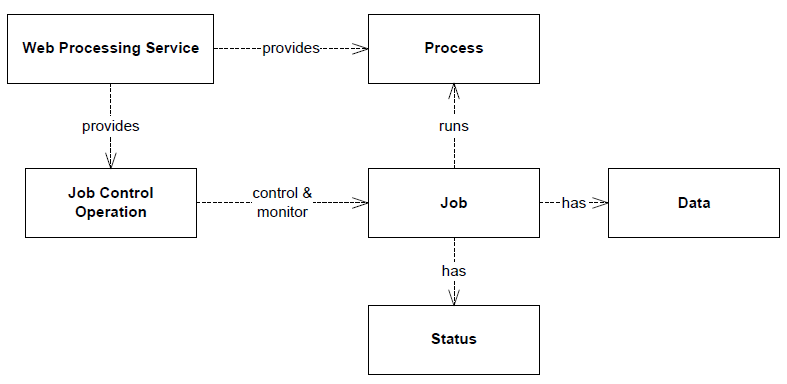
\includegraphics[width=1\linewidth]{UML/WPSmodel.png}
	\caption{Artifacts of the \ac{wps} service model \citep[p. 15]{GEO:OGC}}
	\label{fig:WPSmodel}
\end{figure}

\subsection{Get Capabilities}
\begin{sloppypar}
	All \ac{ogc} web services give an overview of what they have to offer using the so-called \texttt{GetCapabilities} request. The request can be made by taking the \ac{http} address of the \ac{wps} and adding: \url{service=wps&request=getcapabilities} . This returns a document with information about the service metadata, the basic process offerings, and available processes. Figure \ref{fig:WPSmodel2} shows the model of this capabilities document. The service identification section of the document gives a description of the service, including the versions that it supports and potential fees or access constraints. The service provider section gives information about the organisation or people who maintain the \ac{wps} and also includes their contact information. The operations metadata lists the different requests that are implemented in this particular \ac{wps} and the \ac{http} addresses to which the GET and POST requests can be send to. The content section of the capabilities document provides an overview of the available process offerings. For every process an identifier, title and description are listed. Optionally an extensions section can be added that describes additional service capabilities. At the end of the document the language section lists the languages that are supported and the default language that is being used. An example of an capabilities document can be found in Appendix \ref{app:wpsCapabilities}. 
\end{sloppypar}

\begin{figure}
	\centering
	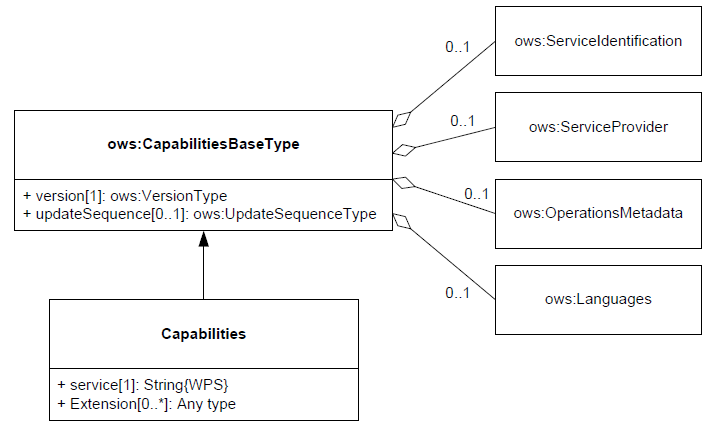
\includegraphics[width=1\linewidth]{UML/WPSmodel2.png}
	\caption{\ac{uml} model of WPS capabilities document \citep[p. 70]{GEO:OGC}}
	\label{fig:WPSmodel2}
\end{figure}

\subsection{Describe Process}
\begin{sloppypar}
A more detailed description of a process listed in the capabilities document of the \ac{wps} can be retrieved using the \texttt{DescribeProcess} request. This request requires the identifier of the process to be passed as a parameter. Optionally, a specific language can be requested for the response document (from the list of available languages in the capabilities document). The process description includes information about input parameters and output data, such as their identifiers, data type, mime types or default values. A describe sensor request can be made by putting the base address of the \ac{wps} and adding: \url{service=wps&version=1.0.0&request=describeprocess&identifier=an_identifier} where the version parameter should be in accordance with the supported version(s) from the capabilities document and the identifier should be taken from the process offerings section of the capabilities document. An example of a describe sensor response document can be found in Appendix \ref{app:wpsDescribe}.  
\end{sloppypar}


\subsection{Execute}
A \ac{wps} process can be started using the \texttt{Execute} request. To make this request the \ac{http} address of the \ac{wps} is extended with: \url{service=wps&version=1.0.0&request=execute&identifier=GetSensors} where the version parameter should be in accordance with the supported version(s) from the capabilities document and the identifier should be taken from the process offerings section of the capabilities document. Additionally, the desired execution mode can be added to the request (synchronous, asynchronous or auto) as well as the desired output format (response document or raw data). By default the execution mode is set to `document'.

\begin{sloppypar}
	Depending on the individual requirements of the process, input parameters can be added using \url{&DataInputs=[parameterName1=value1;parameterName2=value2]}. The parameter names are defined in the describe process response document, as well as the allowed values for each parameter. There are two kinds of input parameters that can be put in a \texttt{Execute} request: literal and complex data inputs. Literal data inputs can be a string of characters in consisting of different data types (e.g. Double, Integer, String), a given value range, and associated units (e.g. meters, degrees Celsius) \citep[p. 36]{GEO:OGC}. 
\end{sloppypar} 

Complex data inputs are made for inputting complex vector-, raster- or other (non-spatial) kind of data. This data can be inserted directly in the request or indirectly by referencing to a file. The process will then first retrieve this file from a remote server before running. A complex data input defines the allowed mime types that the process accepts.  

When the process finishes an `execute response document' is retrieved. This document has a process section with the identifier, title and abstract of the finished process. It also contains a status section with the time the process ended and whether it finished successfully. If any output data has been produced a \textit{ProcessOutputs} section is created that contains the identifiers of the outputs and the corresponding data. An example of an execute response document can be found in Appendix \ref{app:wpsExecute}.

\subsection{Other requests}
\begin{sloppypar}
	\ac{wps} processes can run synchronously or asynchronously. With a synchronous execution the connection with the client stays open until the process has finished. However, for processes that take longer to execute the asynchronous mode is better suited. The process will continue running after the connection has been closed. With a \texttt{GetStatus} request the client can check whether the process is still running. This request is structured the same way as the execute request, but with the mode set to `status'. Once it has finished the \texttt{GetResult} request allows the client to retrieve the output data. The \texttt{Dismiss} request can be made to communicate to the server that the client is no longer interested in the results of a job. This job will then be cancelled and its output deleted. A job identifier is a required parameter for all three of these requests.
\end{sloppypar}
 
